%!TEX encoding = UTF-8 Unicode
%!TEX root = ../lect-week04.tex

\ifkompendium\else
\Subsection{Samlingar}

\begin{Slide}{Vad är en samling?}
En \Emph{samling} \Eng{collection} är en datastruktur som kan innehålla många element av \Alert{samma typ}.
\end{Slide}

\fi

\ifkompendium
\begin{Slide}{Hierarki av samlingar i scala.collection}
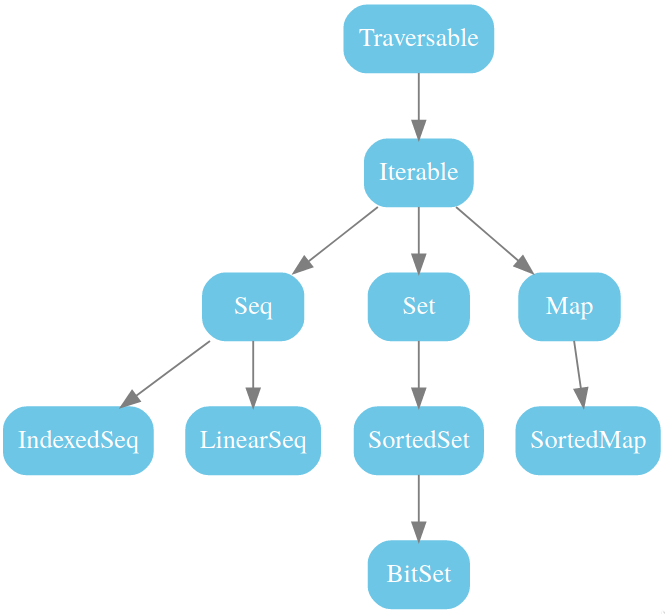
\includegraphics[width=1.0\textwidth]{../img/collection/collection-traits}
\end{Slide}



\noindent Läs mer om Scalas samlingar här: \\ 
\url{http://docs.scala-lang.org/overviews/collections/overview}
\fi

\ifkompendium\else

\begin{Slide}{Hierarki av samlingstyper i \texttt{scala.collection}}

\begin{multicols}{2}
\begin{tikzpicture}[sibling distance=6.1em,->,>=stealth', inner sep=3pt, %scale=0.5, 
  every node/.style = {shape=rectangle, draw, align=center,font=\small\ttfamily},
  class/.style = {fill=blue!20},
  trait/.style = {rounded corners, fill=red!20}]
  \node[trait] {Traversable}
    child { node[trait] {Iterable} 
      child { node[trait] {Seq} 
       }
      child { node[trait] {Set} 
      }
      child { node[trait] {Map} 
      }
    };
\end{tikzpicture}

\columnbreak
 
{\SlideFontTiny 

\code{Traversable} har metoder som är implementerade med hjälp av: \\
\code{def foreach[U](f: Elem => U): Unit}\\

\vspace{1em}\code{Iterable} har metoder som är implementerade med hjälp av: \\
\code{def iterator: Iterator[A] } 

}

\begin{itemize}\SlideFontTiny 
\item[] \code{Seq}: ordnade i sekvens
\item[] \code{Set}: unika element
\item[] \code{Map}: par av (nyckel, värde)
\end{itemize}


\end{multicols}
\end{Slide}

\begin{Slide}{Använda \texttt{iterator}}\SlideFontSmall
Med en \code{iterator} kan man \Emph{iterera} med \code{while} över alla element, men endast \Alert{en   gång}; sedan är iteratorn ''förbrukad''. (Men man kan be om en ny.)
\begin{REPL}
scala> val xs = Vector(1,2,3,4)
xs: scala.collection.immutable.Vector[Int] = Vector(1, 2, 3, 4)

scala> val it = xs.iterator
it: scala.collection.immutable.VectorIterator[Int] = non-empty iterator

scala> while (it.hasNext) print(it.next)
1234

scala> it.hasNext
res1: Boolean = false

scala> it.next
java.util.NoSuchElementException: reached iterator end
  at scala.collection.immutable.VectorIterator.next(Vector.scala:674)
\end{REPL}
\Emph{Normalt} behöver man \Alert{inte} använda \code{iterator}, utan det finns färdiga metoder som gör det man vill, till exempel \code{foreach}, \code{map}, \code{sum}, \code{min} etc.
\end{Slide}

\begin{Slide}{Några användbara metoder på samlingar}\SlideFontTiny
\begin{tabular}{r r l}
\texttt{\Emph{Traversable}} & & \\
  & \code|xs.size| & antal elementet \\
  & \code|xs.head| & första elementet \\
  & \code|xs.last| & sista elementet \\
  & \code|xs.take(n)| & ny samling med de första n elementet \\
  & \code|xs.drop(n)| & ny samling utan de första n elementet \\
  & \code|xs.foreach(f)| & gör \code|f| på alla element, returtyp \code|Unit|\\
  & \code|xs.map(f)| & gör \code|f| på alla element, ger \Alert{ny} samling \\
  
\texttt{\Emph{Iterable}} & & \\
  & \code|xs.zip(ys)| & ny samling med par (x, y); ''zippa ihop'' xs och ys \\
  & \code|xs.zipWithIndex| & ny samling med par (x, index för x) \\
  & \code|xs.sliding(n)| & ny samling av samlingar genom glidande ''fönster''\\

\texttt{\Emph{Seq}} & & \\
  & \code|xs.length| & samma som \code|xs.size| \\
  & \code|xs :+ x| & ny samling med x sist efter xs \\
  & \code|x +: xs| & ny samling med x före xs \\
  
\end{tabular}

\pause
\vspace{1em}\Emph{Minnesregel} för \code{+:} och \code{:+  } \Alert{Colon on the collection side}

\pause
\vspace{1em} Prova fler samlingsmetoder genom att noga studera \url{http://cs.lth.se/quickref}
\end{Slide}

\begin{Slide}{Mer specifik samlingstyper i \texttt{scala.collection}}
Det finns mer specifika \Emph{subtyper} av \code{Seq}, \code{Set} och \code{Map}:
\\ \vspace{1em}

\begin{tikzpicture}[sibling distance=5.8em,->,>=stealth', inner sep=3pt, %scale=0.5, 
  every node/.style = {shape=rectangle, draw, align=center,font=\small\ttfamily},
  class/.style = {fill=blue!20},
  trait/.style = {rounded corners, fill=red!20}]
  \node[trait] {Traversable}
    child { node[trait] {Iterable} 
      child { node[trait, xshift=-2.4cm] {Seq} 
        child { node[trait] {IndexedSeq} }
        child { node[trait] {LinearSeq} }
       }
      child { node[trait, yshift=-0.0cm] {Set} 
        child { node[trait] {SortedSet} }
        child { node[trait] {BitSet} }
      }
      child { node[trait, xshift=1.0cm] {Map} 
        child { node[trait] {SortedMap} }
      }
    };
\end{tikzpicture}

\vspace{0.5em}
\Emph{\texttt{Vector}} är en \code{IndexedSeq} medan
\Emph{\texttt{List}} är en \code{LinearSeq}.
\end{Slide}

\begin{Slide}{Några oföränderliga och förändringsbara sekvenssamlingar}\SlideFontSmall
\begin{tabular}{r l l}
\texttt{scala.collection.\Emph{immutable}.Seq.} & & \\
 & \code|IndexedSeq.| & \\
 & & \Emph{\texttt{Vector}} \\
 & & \Emph{\texttt{Range}} \\
 & \code|LinearSeq.| & \\
 & & \Emph{\texttt{List}} \\
   & & \Emph{\texttt{Queue}} \\

\texttt{scala.collection.\Alert{mutable}.Seq.} & & \\
 & \code|IndexedSeq.| & \\
 & & \Alert{\texttt{ArrayBuffer}} \\
 & & \Alert{\texttt{StringBuilder}} \\
 & \code|LinearSeq.| & \\
 & & \Alert{\texttt{ListBuffer}} \\
   & & \Alert{\texttt{Queue}} \\
\end{tabular}

Studera samlingars egenskaper här: \href{http://docs.scala-lang.org/overviews/collections/overview}{docs.scala-lang.org/overviews/collections/overview}
\end{Slide}


\begin{Slide}{scala.collection.immutable}
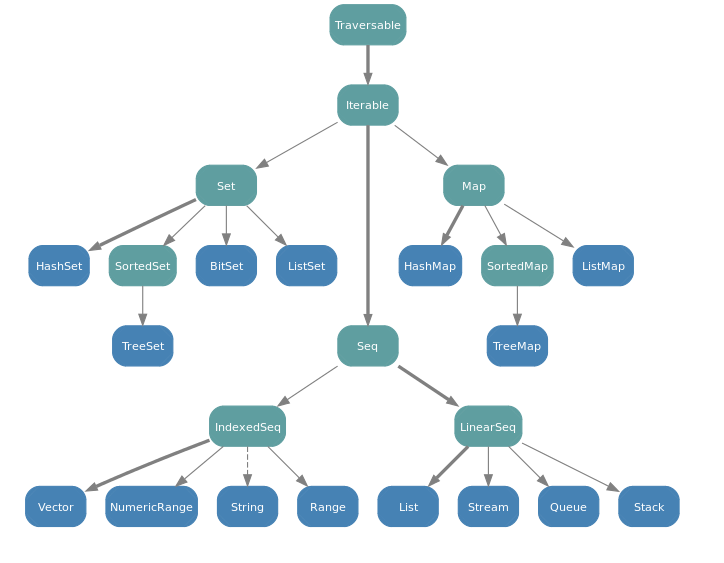
\includegraphics[width=0.82\textwidth]{../img/collection/collection-immutable}
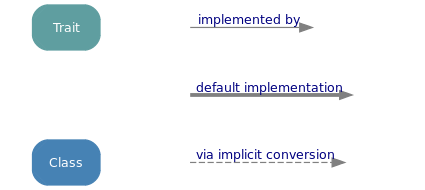
\includegraphics[width=0.33\textwidth]{../img/collection/collection-legend}
\end{Slide}

\begin{Slide}{scala.collection.mutable}
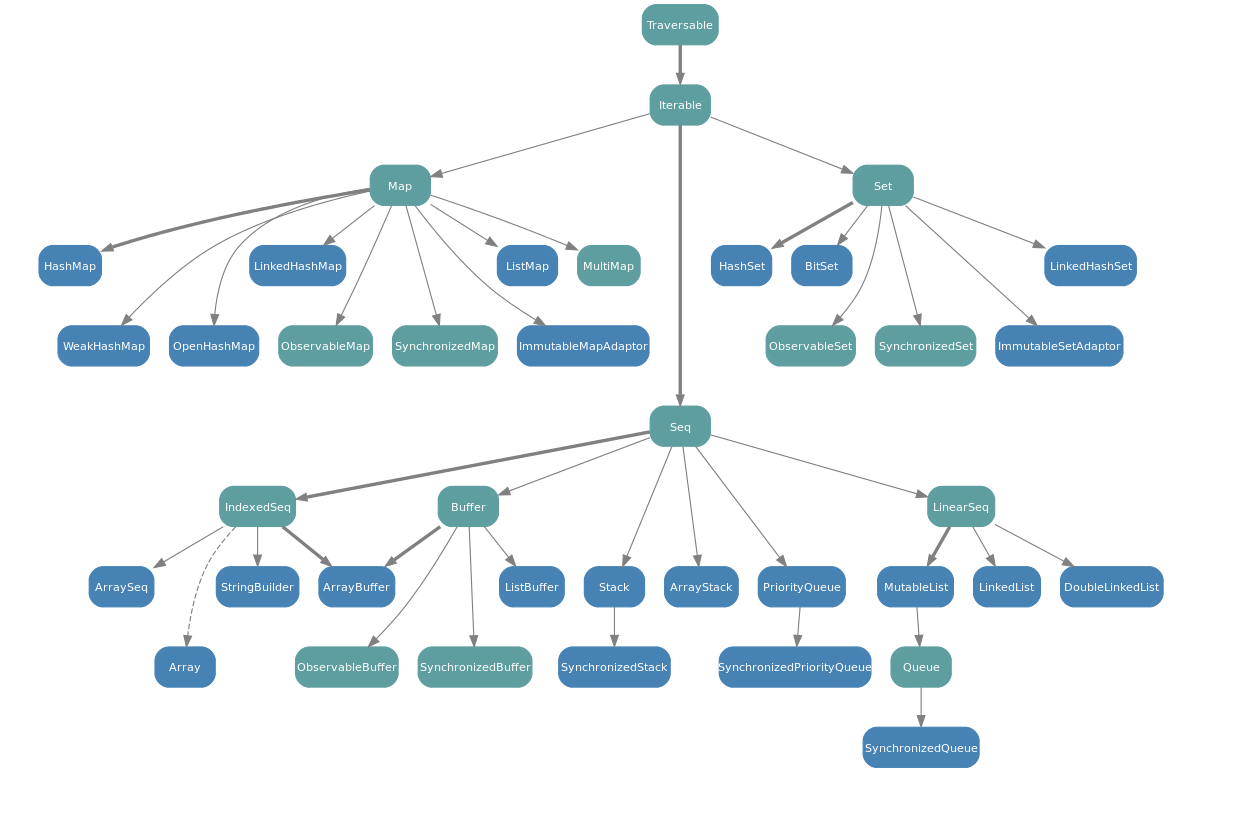
\includegraphics[width=1.05\textwidth]{../img/collection/collection-mutable}
\end{Slide}


\begin{Slide}{\texttt{Vector} eller \texttt{List}?}\SlideFontTiny
{\href{http://stackoverflow.com/questions/6928327/when-should-i-choose-vector-in-scala}{stackoverflow.com/questions/6928327/when-should-i-choose-vector-in-scala}}

\begin{itemize}
\item If we only need to transform sequences by operations like map, filter, fold etc: basically it does not matter, we should program our algorithm generically and might even benefit from accepting parallel sequences. For sequential operations List is probably a bit faster. But you should benchmark it if you have to optimize.

\item If we need a lot of random access and different updates, so we should use vector, list will be prohibitively slow.

\item If we operate on lists in a classical functional way, building them by prepending and iterating by recursive decomposition: use list, vector will be slower by a factor 10-100 or more.

\item If we have an performance critical algorithm that is basically imperative and does a lot of random access on a list, something like in place quick-sort: use an imperative data structure, e.g. ArrayBuffer, locally and copy your data from and to it.
\end{itemize}
{\href{http://stackoverflow.com/questions/20612729/how-does-scalas-vector-work}{stackoverflow.com/questions/20612729/how-does-scalas-vector-work}}\\
Mer om tids- och minneskomplexitet i fördjupningskursen och senare kurser.
\end{Slide}

\begin{Slide}{Speciella metoder på förändringsbara samlingar}
\end{Slide}


\begin{Slide}{Mängd för snabb innehållstest, granterat dublettfri}
\end{Slide}

\begin{Slide}{Den fantastiska nyckel-värde-tabellen \texttt{Map}}
\end{Slide}


\fi






